\documentclass[tikz,border=12pt]{standalone}
\usepackage[T1]{fontenc}
\usepackage{lmodern,amsmath,amssymb}
\usetikzlibrary{arrows.meta,positioning}
\definecolor{ink}{HTML}{183444}
\definecolor{blue}{HTML}{1B6780}
\definecolor{amber}{HTML}{AD601A}
\begin{document}
\hyphenpenalty=10000\exhyphenpenalty=10000
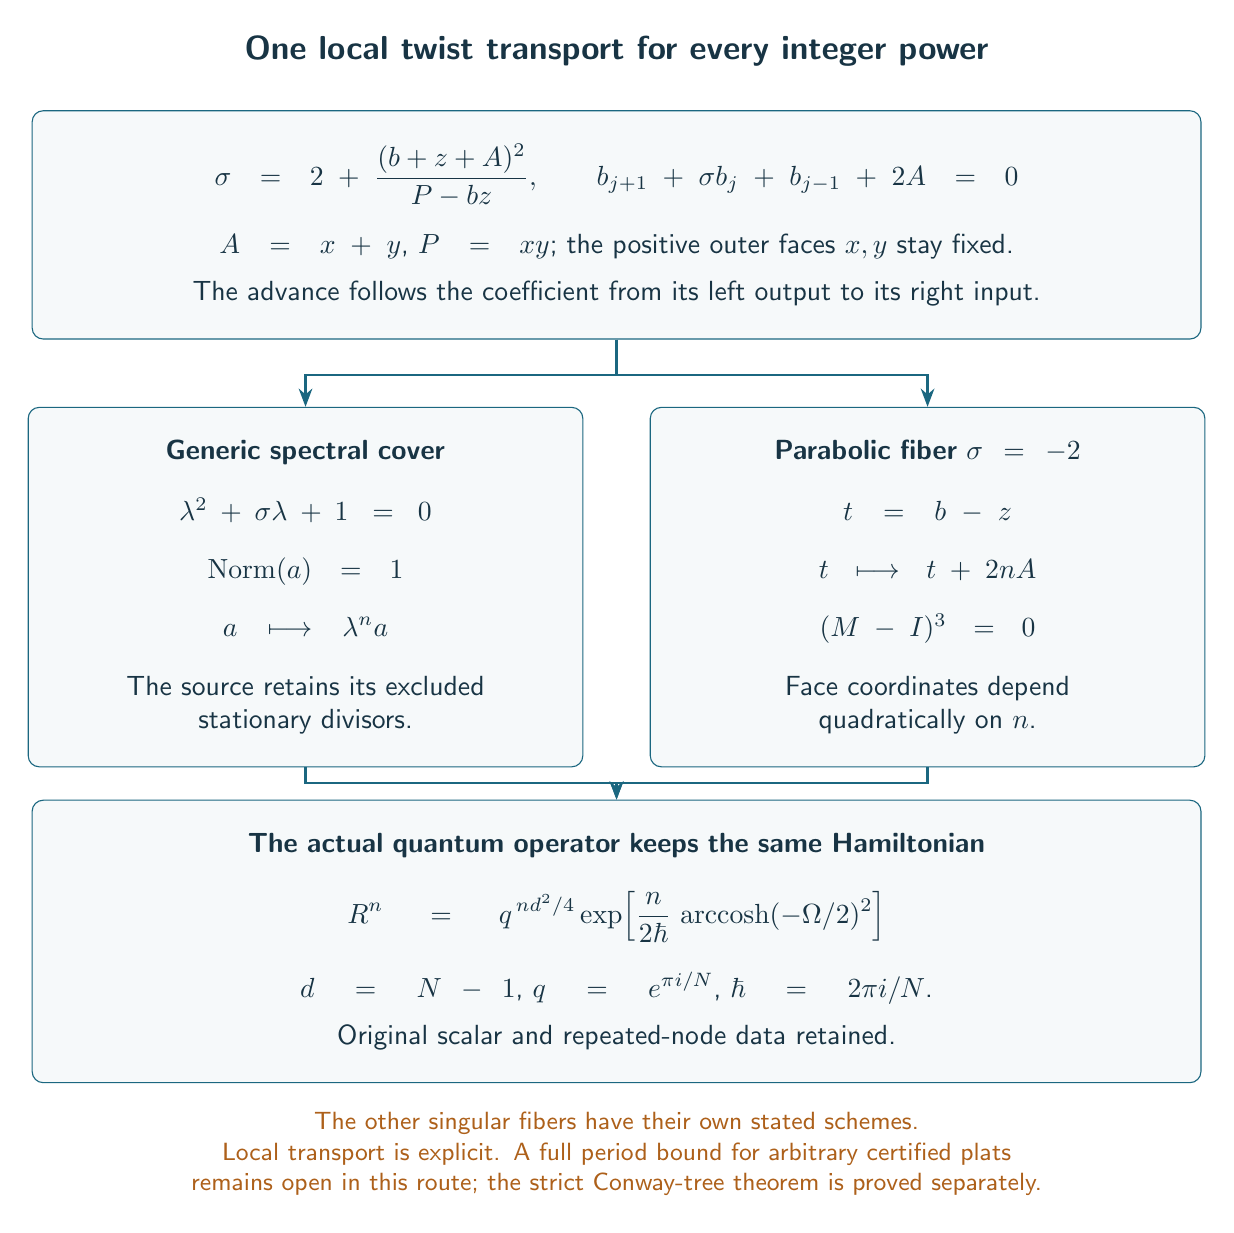
\begin{tikzpicture}[font=\sffamily,text=ink,>=Stealth,
 panel/.style={draw=blue,fill=blue!4,rounded corners,align=center,inner sep=12pt}]
 \node[font=\sffamily\large\bfseries] at (0,2.2)
 {One local twist transport for every integer power};
 \node[panel,text width=14cm] (source) at (0,0)
 {$\displaystyle \sigma=2+\frac{(b+z+A)^2}{P-bz},\qquad
          b_{j+1}+\sigma b_j+b_{j-1}+2A=0$\\[9pt]
 $A=x+y$, $P=xy$; the positive outer faces $x,y$ stay fixed.\\[5pt]
 The advance follows the coefficient from its left output to its right input.};
 \node[panel,text width=6.2cm] (torus) at (-3.95,-4.6)
 {\textbf{Generic spectral cover}\\[10pt]
 $\lambda^2+\sigma\lambda+1=0$\\[9pt]
 $\operatorname{Norm}(a)=1$\\[9pt]
 $\displaystyle a\longmapsto\lambda^n a$\\[9pt]
 The source retains its excluded\\stationary divisors.};
 \node[panel,text width=6.2cm] (parabola) at (3.95,-4.6)
 {\textbf{Parabolic fiber $\sigma=-2$}\\[10pt]
 $t=b-z$\\[9pt]
 $\displaystyle t\longmapsto t+2nA$\\[9pt]
 $(M-I)^3=0$\\[9pt]
 Face coordinates depend\\quadratically on $n$.};
 \draw[->,blue,thick] (source.south)--++(0,-.45)-|(torus.north);
 \draw[->,blue,thick] (source.south)--++(0,-.45)-|(parabola.north);
 \node[panel,text width=14cm] (quantum) at (0,-9.1)
 {\textbf{The actual quantum operator keeps the same Hamiltonian}\\[11pt]
 $\displaystyle R^n=q^{\,nd^2/4}
     \exp\!\left[\frac{n}{2\hbar}\,\operatorname{arccosh}(-\Omega/2)^2\right]$\\[10pt]
 $d=N-1$, $q=e^{\pi i/N}$, $\hbar=2\pi i/N$.\\[5pt]
 Original scalar and repeated-node data retained.};
 \draw[->,blue,thick] (torus.south)--++(0,-.2)-|(quantum.north);
 \draw[->,blue,thick] (parabola.south)--++(0,-.2)-|(quantum.north);
 \node[amber,align=center,text width=14cm,font=\sffamily\small] at (0,-11.8)
 {The other singular fibers have their own stated schemes.\\
 Local transport is explicit. A full period bound for arbitrary certified plats\\
 remains open in this route; the strict Conway-tree theorem is proved separately.};
\end{tikzpicture}
\end{document}
